\def\mytitle{ASSIGNMENT-1}
\def\myauthor{Gajula Arun Kumar}
\def\contact{arunkumarg099@gmail.com}
\def\mymodule{Future Wireless Communications (FWC)}
\documentclass[10pt, a4paper]{article}
\usepackage[a4paper,outer=1.5cm,inner=1.5cm,top=1.75cm,bottom=1.5cm]{geometry}
\twocolumn
\usepackage{graphicx}
\graphicspath{{./images/}}
\usepackage[colorlinks,linkcolor={black},citecolor={blue!80!black},urlcolor={blue!80!black}]{hyperref}
\usepackage[parfill]{parskip}
\usepackage{lmodern}
\usepackage{tikz}

\usepackage{karnaugh-map}

\usepackage{tabularx}
%\documentclass{article}
%\documentclass[tikz, border=2mm]{standalone}
%\usepackage{tikz}
%\usepackage{circuitikz}
\usetikzlibrary{calc}

\renewcommand*\familydefault{\sfdefault}
\usepackage{watermark}
\usepackage{lipsum}
\usepackage{xcolor}
\usepackage{listings}
\usepackage{float}
\usepackage{titlesec}

\titlespacing{\subsection}{1pt}{\parskip}{3pt}
\titlespacing{\subsubsection}{0pt}{\parskip}{-\parskip}
\titlespacing{\paragraph}{0pt}{\parskip}{\parskip}
\newcommand{\figuremacro}[5]{
    \begin{figure}[#1]
        \centering
        \includegraphics[width=#5\columnwidth]{#2}
        \caption[#3]{\textbf{#3}#4}
        \label{fig:#2}
    \end{figure}
}

\lstset{
frame=single, 
breaklines=true,
columns=fullflexible
}

%\thiswatermark{\centering \put(400,-128.0){\includegraphics[scale=0.3]{logo}} }
\title{\mytitle}
\author{\myauthor\hspace{1em}\\\contact\\IITH\hspace{0.5em}-\hspace{0.6em}\mymodule}
\date{20-12-2022}
\begin{document}
  \maketitle
  \tableofcontents
  \begin{abstract}
      This manual explains about a logic circiut which implements the boolean function F=X'Y+XY'Z', where the input combination X=Y=1 can never occur. Finding the simplified expression of F:
%\figuremacro{h}{diag}{}{}{0.9}
  \end{abstract}


  \section{Components}
  \begin{tabularx}{0.4\textwidth} { 
  | >{\centering\arraybackslash}X 
  | >{\centering\arraybackslash}X 
  | >{\centering\arraybackslash}X
  | >{\centering\arraybackslash}X | }
\hline
 \textbf{Component}& \textbf{Values} & \textbf{Quantity}\\
\hline
Arduino & UNO & 1 \\  
\hline
JumperWires& M-M & 10 \\ 
\hline
Breadboard &  & 1 \\
\hline
LED & &2 \\
\hline
Resistor &220ohms & 1\\
\hline
\end{tabularx}



\begin{center}
Figure.a
\end{center}

\section{Truth Table}
  \begin{tabularx}{0.46\textwidth} { 
  | >{\centering\arraybackslash}X 
  | >{\centering\arraybackslash}X 
  | >{\centering\arraybackslash}X
  | >{\centering\arraybackslash}X 
  | >{\centering\arraybackslash}X 
  | >{\centering\arraybackslash}X 
  | >{\centering\arraybackslash}X 
  | >{\centering\arraybackslash}X 
  | >{\centering\arraybackslash}X 
  | >{\centering\arraybackslash}X | }


\hline
\textbf{X} & \textbf{Y} & \textbf{Z} & \textbf{F}\\
\hline
0 & 0 & 0 & 0  \\  
\hline
0 & 0 & 1 & 0  \\ 
\hline
0 & 1 & 0 & 0  \\
\hline
0 & 1 & 1 & 1  \\
\hline
1 & 0 & 0 & 1  \\  
\hline
1 & 0 & 1 & 0  \\ 
\hline
1 & 1 & 0 & -  \\
\hline
1 & 1 & 1 & -  \\
\hline
\end{tabularx}
\begin{center}
 Truth table Boolean Function "F"
\end{center}


\section{K-map Implementation}
\begin{center}
    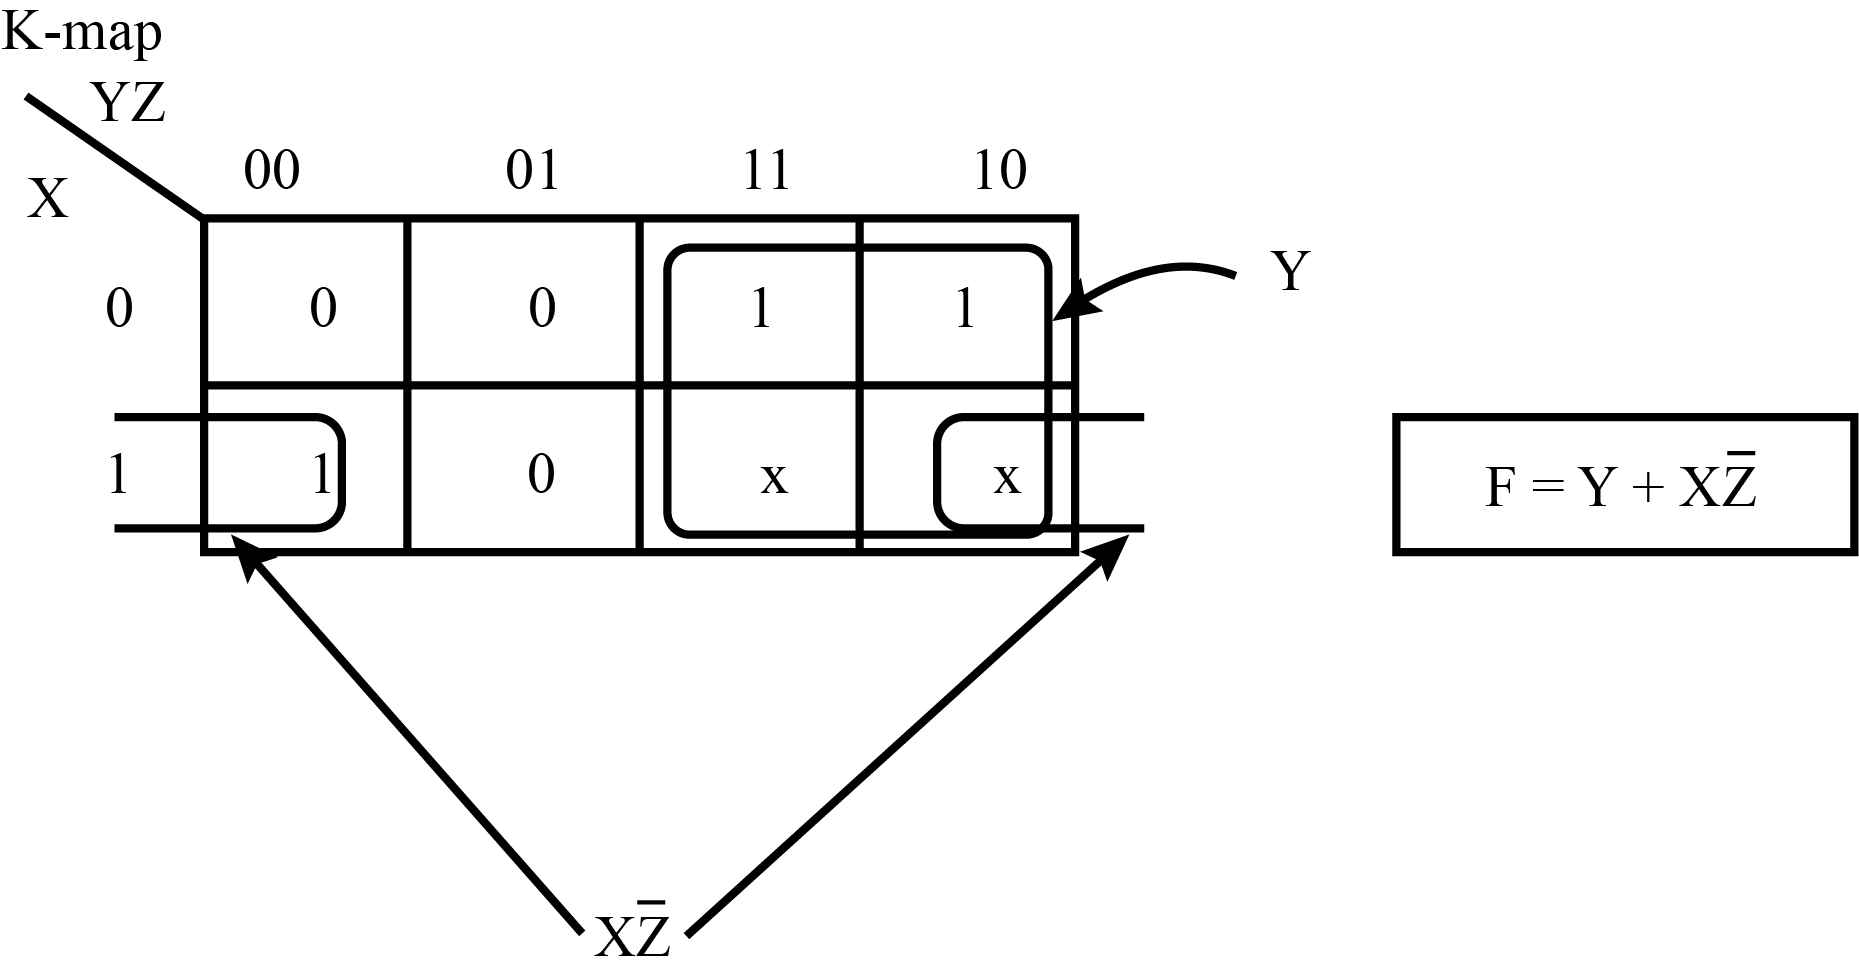
\includegraphics[scale=0.5]{img.png}
\end{center}


 \paragraph {Reducing the boolean Function}:\\
    F=X'Y+XY'Z'\\
    F=X'Y(Z+Z')+XY'Z'\\
    X'YZ+X'YZ'+XY'Z'\\
 Reduced expression using K-maps is\\
 F=Y+XZ'\\

    
\section{Implementation}
  \begin{tabularx}{0.46\textwidth} { 
  | >{\centering\arraybackslash}X 
  | >{\centering\arraybackslash}X 
  | >{\centering\arraybackslash}X
  | >{\centering\arraybackslash}X 
  | >{\centering\arraybackslash}X 
  | >{\centering\arraybackslash}X 
  | >{\centering\arraybackslash}X 
  | >{\centering\arraybackslash}X 
  | >{\centering\arraybackslash}X
  | >{\centering\arraybackslash}X
  | >{\centering\arraybackslash}X
  | >{\centering\arraybackslash}X
  | >{\centering\arraybackslash}X
  | >{\centering\arraybackslash}X
  | >{\centering\arraybackslash}X 
  | >{\centering\arraybackslash}X | }


\hline
\textbf{Arduino PIN} & \textbf{INPUT} & \textbf{OUTPUT} \\ 
\hline
\textbf 2 & X & \\
\hline
\textbf 3 & Y & \\
\hline
\textbf 4 & Z & \\
\hline
\textbf 8 & & F \\
\hline
\end{tabularx}

\begin{center}
    Connections
\end{center}

    \paragraph{Problem-1}:\\
    
    1. Connect the circuit as per the above table.\\
    2. Connect the output pin to LED\\
    3. Execute the circuit using the below code.\\

   \paragraph{Problem-2}:\\
1. Change the values of X,Y,Z in the code and verify the Truth Table\\


\bibliographystyle{ieeetr}
\end{document}